\documentclass{beamer}

\usepackage{tikz}
\usetikzlibrary{calc,backgrounds}
\usepackage{amsmath}
\usepackage{amssymb}
\usepackage{float}
\usepackage{graphicx}
\usepackage{svg}
\usepackage{pgfplots}
\usepackage{xcolor}
\usepackage{subcaption}

\usetikzlibrary{fadings}
\tikzfading
  [name=fadeLR,
   left color=transparent!100,  % fully transparent at the left
   right color=transparent!0]   % fully opaque at the right
\tikzfading
   [name=fadeRL,
    right color=transparent!100,  % fully transparent at the left
    left color=transparent!0]   % fully opaque at the right

\definecolor{pale_yellow}{HTML}{ffef96}

\definecolor{col1}{HTML}{7570B3}
\definecolor{col2}{HTML}{D95F02}
\definecolor{col3}{HTML}{1B9E77}
\definecolor{col4}{HTML}{E7298A}
\definecolor{col5}{HTML}{66A61E}
\definecolor{col6}{HTML}{E6AB02}

\title{Ordinally Partitioned Echo State Networks}% TODO title
\author{Hector Morlet\\22247737}
\date{March 14, 2025}

\begin{document}

\frame{\titlepage} % Title slide

\begin{frame}
    \frametitle{Agenda}
    \begin{itemize}
        \item Introduction to Echo State Networks
        \item Introduction to Ordinal Partitions
        \item Research Proposal
        \item Implementation
        \item Testing and Evaluation
        \item Results and Analysis
        \item Conclusion and Upcoming Work
    \end{itemize}
\end{frame}

\begin{frame}
    \frametitle{Echo State Networks}

    Reservoir computing
\end{frame}

\begin{frame}
    \frametitle{Echo State Networks}

    \begin{figure}
        
    %     \centering
        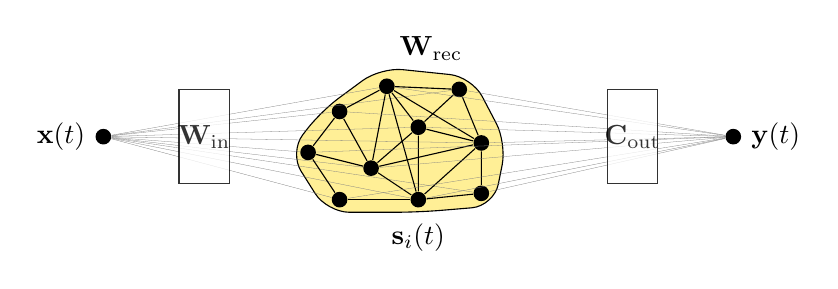
\begin{tikzpicture}[scale=0.8]
            \node[fill=black,circle,inner sep=2pt,label=left:$\mathbf{x}(t)$] (input) at (0,0) {};
            \node[fill=black,circle,inner sep=2pt,label=right:$\mathbf{y}(t)$] (output) at (10,0) {};
            
            
            \coordinate (res_anchor) at (2,3);
            \node[fill=black,circle,inner sep=2pt] (res1) at ({5-0.5},{0.8}) {};
            \node[fill=black,circle,inner sep=2pt] (res2) at ({5},{-1}) {};
            \node[fill=black,circle,inner sep=2pt] (res3) at ({5},{0.15}) {};
            \node[fill=black,circle,inner sep=2pt] (res4) at ({5+1},{-0.1}) {};
            \node[fill=black,circle,inner sep=2pt] (res5) at ({5-0.75},{-0.5}) {};
            \node[fill=black,circle,inner sep=2pt] (res6) at ({5-1.25},{0.4}) {};
            \node[fill=black,circle,inner sep=2pt] (res7) at ({5+0.65},{0.75}) {};
            \node[fill=black,circle,inner sep=2pt] (res8) at ({5+1},{-0.9}) {};
            \node[fill=black,circle,inner sep=2pt] (res9) at ({5-1.25},{-1}) {};
            \node[fill=black,circle,inner sep=2pt] (res10) at ({5-1.75},{-0.25}) {};
        
            \foreach \i in {1,...,10}
                \draw[gray,line width=0.1] (input) -- (res\i);
            
            \foreach \i in {1,...,5}
                \foreach \j in {1,...,5} {
                    \ifnum\i<\j
                        \draw (res\i) -- (res\j);
                    \fi
                }
            
            \draw (res6) -- (res5);
            \draw (res6) -- (res1);
            \draw (res6) -- (res10);
            \draw (res10) -- (res5);
            \draw (res9) -- (res10);
            \draw (res9) -- (res2);
            \draw (res7) -- (res1);
            \draw (res7) -- (res3);
            \draw (res7) -- (res4);
            \draw (res8) -- (res4);
            \draw (res8) -- (res2);
            
            \foreach \i in {1,...,10}
                \draw[gray,line width=0.1] (res\i) -- (output);
            
            \begin{scope}[on background layer]
            \draw[draw=black,fill=pale_yellow,rounded corners=8pt]  ($(res1)+(-0.1,0.3)$) -- ($(res7)+(+0.2,+0.2)$) -- ($(res4)+(0.4,0)$) -- ($(res8)+(0.2,-0.2)$) -- ($(res2)+(0,-0.2)$) -- ($(res9)+(-0.2,-0.2)$) -- ($(res10)+(-0.3,0)$) -- ($(res6)+(-0.3,0)$) -- cycle;
            \end{scope}
            \node at (5.2, 1.4) {$\mathbf{W}_{\text{rec}}$};
            \node at (5, -1.6) {$\mathbf{s}_i(t)$};
            
            \draw[fill=white,opacity=0.8] (1.2,-0.75) rectangle (2.0,0.75) node[midway] {$\mathbf{W}_{\text{in}}$};
            \draw[fill=white,opacity=0.8] (8, -0.75) rectangle (8.8,0.75) node[midway] {$\mathbf{C}_{\text{out}}$};
        \end{tikzpicture}
        \caption{A diagram of an Echo State Network.}
        \label{fig:ESN}
    \end{figure}
\end{frame}

\begin{frame}
    \frametitle{Ordinal Partitions}

    \begin{itemize}
        \item Each point in a timeseries is categorised by the ranking of its preceding points.
    \end{itemize}
    
    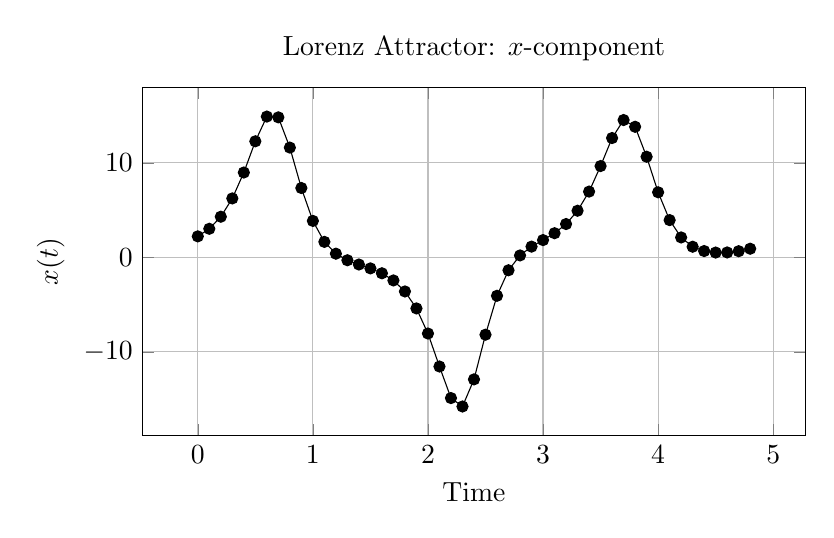
\begin{tikzpicture}
        \begin{axis}[
          xlabel={Time},
          ylabel={$x(t)$},
          title={Lorenz Attractor: $x$-component},
          width=10cm, height=6cm,
          grid=major
        ]
          % Data generated by solving dx/dt = sigma(y - x), etc. in Python
          \addplot[black, mark=*, mark options={black}] coordinates {
            (0.0, 2.2165566502619796)
            (0.1, 3.0181360987381685)
            (0.2, 4.2948078524935065)
            (0.3, 6.231121537780632)
            (0.4, 8.970926893912857)
            (0.5, 12.272230400810887)
            (0.6, 14.887997312478161)
            (0.7, 14.803117347063516)
            (0.8, 11.606868473299526)
            (0.9, 7.330990437181266)
            (1.0, 3.85191889651296)
            (1.1, 1.6347534154776406)
            (1.2, 0.3853895148599277)
            (1.3, -0.30838099414996695)
            (1.4, -0.7586726217449103)
            (1.5, -1.1695821908357407)
            (1.6, -1.6858338981790886)
            (1.7, -2.443141458426554)
            (1.8, -3.6086854451117074)
            (1.9, -5.40339197322587)
            (2.0, -8.058505977971057)
            (2.1, -11.547145254692042)
            (2.2, -14.884182443761347)
            (2.3, -15.775516623377253)
            (2.4, -12.908181797239536)
            (2.5, -8.181376578133673)
            (2.6, -4.06724026097539)
            (2.7, -1.3665393788429014)
            (2.8, 0.20110496364168012)
            (2.9, 1.1324784341364973)
            (3.0, 1.8245674314417792)
            (3.1, 2.5516132966355554)
            (3.2, 3.5214281335608555)
            (3.3, 4.926987945369609)
            (3.4, 6.951562500713474)
            (3.5, 9.654345729238477)
            (3.6, 12.617195234374243)
            (3.7, 14.521825487882024)
            (3.8, 13.806356286601272)
            (3.9, 10.64113968132102)
            (4.0, 6.880279139891668)
            (4.1, 3.9367704788159394)
            (4.2, 2.1029851064946445)
            (4.3, 1.121305395878461)
            (4.4, 0.665491176850325)
            (4.5, 0.5051437108082056)
            (4.6, 0.5156168027361644)
            (4.7, 0.6490783162490397)
            (4.8, 0.9105168761220792)
          };
        \end{axis}
      \end{tikzpicture}    
\end{frame}

\begin{frame}
    \frametitle{Ordinal Partitions}

    \begin{center}
        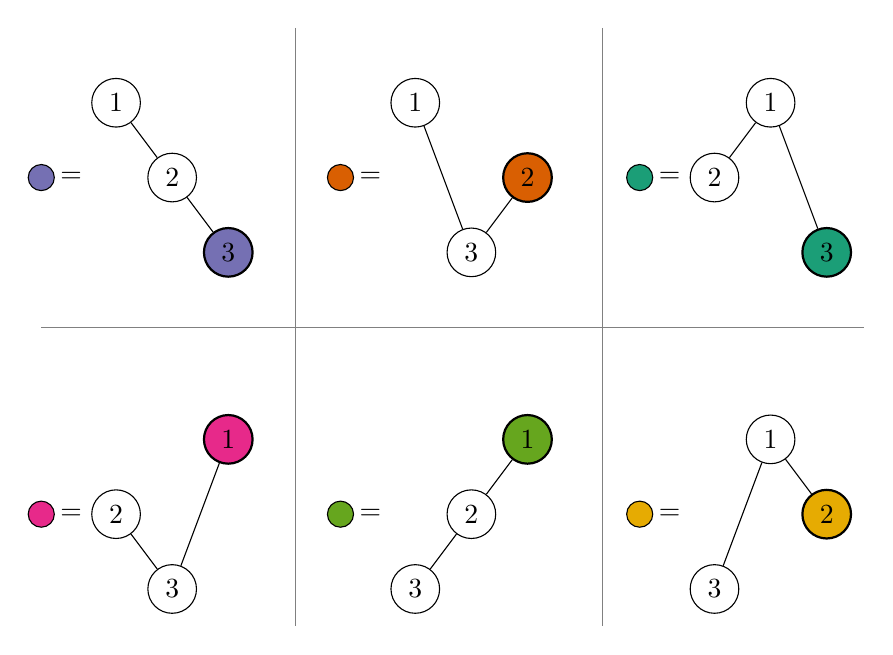
\begin{tikzpicture}[scale=0.95]
            % partition 1

            \node[circle, draw, fill=col1] (topleft) at (-5.0, 3) {};

            % Draw the equality sign
            \node at (-4.6, 3) {$=$};
            
            % Draw the nodes in the lower part
            \node[circle, draw] (1_2) at (-4.0, 4) {1};
            \node[circle, draw] (1_1) at (-3.25, 3) {2};
            \node[circle, draw, thick, fill=col1] (1_3) at (-2.5, 2) {3};
            
            % Draw edges
            \draw (1_1) -- (1_2);
            \draw (1_1) -- (1_3);

            % Draw dividing line
            \draw[gray, very thin] (-1.6, 5) -- (-1.6, -3);

            % partition 2

            \node[circle, draw, fill=col2] (topcentre) at (-1, 3) {};

            % Draw the equality sign
            \node at (-0.6, 3) {$=$};
            
            % Draw the nodes in the lower part
            \node[circle, draw] (2_2) at (0, 4) {1};
            \node[circle, draw] (2_1) at (0.75, 2) {3};
            \node[circle, draw, thick, fill=col2] (2_3) at (1.5, 3) {2};
            
            % Draw edges
            \draw (2_1) -- (2_2);
            \draw (2_1) -- (2_3);

            % Draw dividing line
            \draw[gray, very thin] (2.5, 5) -- (2.5, -3);

            % partition 3

            \node[circle, draw, fill=col3] (topleft) at (3.0, 3) {};

            % Draw the equality sign
            \node at (3.4, 3) {$=$};
            
            % Draw the nodes in the lower part
            \node[circle, draw] (3_2) at (4.0, 3) {2};
            \node[circle, draw] (3_1) at (4.75, 4) {1};
            \node[circle, draw, thick, fill=col3] (3_3) at (5.5, 2) {3};
            
            % Draw edges
            \draw (3_1) -- (3_2);
            \draw (3_1) -- (3_3);

            % Draw dividing line
            \draw[gray, very thin] (-5, 1) -- (6, 1);

            % partition 4

            \node[circle, draw, fill=col4] (bottomleft) at (-5.0, -1.5) {};

            % Draw the equality sign
            \node at (-4.6, -1.5) {$=$};
            
            % Draw the nodes in the lower part
            \node[circle, draw] (4_2) at (-4.0, -1.5) {2};
            \node[circle, draw] (4_1) at (-3.25, -2.5) {3};
            \node[circle, draw, thick, fill=col4] (4_3) at (-2.5, -0.5) {1};
            
            % Draw edges
            \draw (4_1) -- (4_2);
            \draw (4_1) -- (4_3);

            % Draw dividing line
            % \draw[gray, very thin] (-2.25, -3) -- (-2.25, -5);

            % partition 5

            \node[circle, draw, fill=col5] (bottomcentre) at (-1, -1.5) {};

            % Draw the equality sign
            \node at (-0.6, -1.5) {$=$};
            
            % Draw the nodes in the lower part
            \node[circle, draw] (5_2) at (0, -2.5) {3};
            \node[circle, draw] (5_1) at (0.75, -1.5) {2};
            \node[circle, draw, thick, fill=col5] (5_3) at (1.5, -0.5) {1};
            
            % Draw edges
            \draw (5_1) -- (5_2);
            \draw (5_1) -- (5_3);

            % partition 6

            \node[circle, draw, fill=col6] (bottomright) at (3.0, -1.5) {};

            % Draw the equality sign
            \node at (3.4, -1.5) {$=$};
            
            % Draw the nodes in the lower part
            \node[circle, draw] (6_2) at (4.0, -2.5) {3};
            \node[circle, draw] (6_1) at (4.75, -0.5) {1};
            \node[circle, draw, thick, fill=col6] (6_3) at (5.5, -1.5) {2};
            
            % Draw edges
            \draw (6_1) -- (6_2);
            \draw (6_1) -- (6_3);
        \end{tikzpicture}
    \end{center}
\end{frame}

\begin{frame}
    \frametitle{Ordinal Partitions}
    
      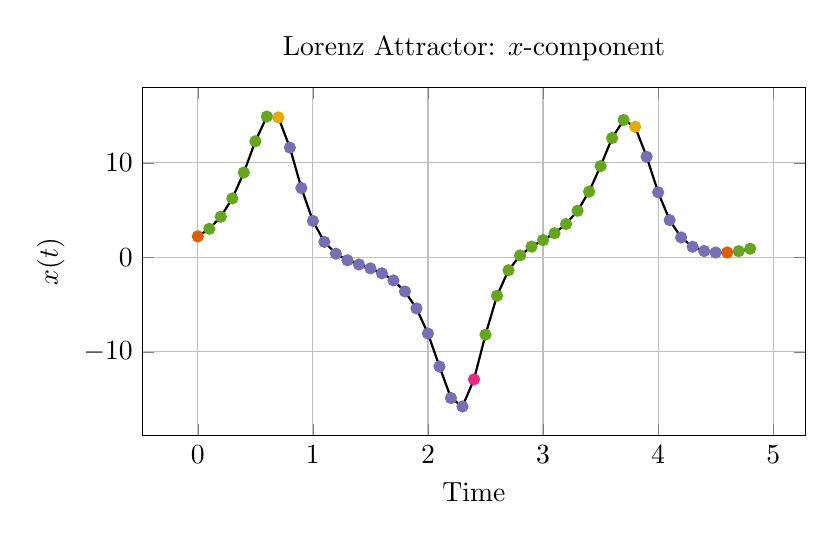
\begin{tikzpicture}
        \begin{axis}[
            xlabel={Time},
            ylabel={$x(t)$},
            title={Lorenz Attractor: $x$-component},
            width=10cm, height=6cm,
            grid=major
        ]


        \addplot [
            thick, % or any style you like
        ] coordinates {
            (0.0, 2.2165566502619796)
            (0.1, 3.0181360987381685)
            (0.2, 4.2948078524935065)
            (0.3, 6.231121537780632)
            (0.4, 8.970926893912857)
            (0.5, 12.272230400810887)
            (0.6, 14.887997312478161)
            (0.7, 14.803117347063516)
            (0.8, 11.606868473299526)
            (0.9, 7.330990437181266)
            (1.0, 3.85191889651296)
            (1.1, 1.6347534154776406)
            (1.2, 0.3853895148599277)
            (1.3, -0.30838099414996695)
            (1.4, -0.7586726217449103)
            (1.5, -1.1695821908357407)
            (1.6, -1.6858338981790886)
            (1.7, -2.443141458426554)
            (1.8, -3.6086854451117074)
            (1.9, -5.40339197322587)
            (2.0, -8.058505977971057)
            (2.1, -11.547145254692042)
            (2.2, -14.884182443761347)
            (2.3, -15.775516623377253)
            (2.4, -12.908181797239536)
            (2.5, -8.181376578133673)
            (2.6, -4.06724026097539)
            (2.7, -1.3665393788429014)
            (2.8, 0.20110496364168012)
            (2.9, 1.1324784341364973)
            (3.0, 1.8245674314417792)
            (3.1, 2.5516132966355554)
            (3.2, 3.5214281335608555)
            (3.3, 4.926987945369609)
            (3.4, 6.951562500713474)
            (3.5, 9.654345729238477)
            (3.6, 12.617195234374243)
            (3.7, 14.521825487882024)
            (3.8, 13.806356286601272)
            (3.9, 10.64113968132102)
            (4.0, 6.880279139891668)
            (4.1, 3.9367704788159394)
            (4.2, 2.1029851064946445)
            (4.3, 1.121305395878461)
            (4.4, 0.665491176850325)
            (4.5, 0.5051437108082056)
            (4.6, 0.5156168027361644)
            (4.7, 0.6490783162490397)
            (4.8, 0.9105168761220792)
        };
        
        
        % Define how each "class" (symbolic label) is colored and drawn:
        \addplot[
            scatter,
            only marks,
            scatter src=explicit symbolic,
            scatter/classes={
                1={mark=*,draw=col1,fill=col1},
                2={mark=*,draw=col2,fill=col2},
                3={mark=*,draw=col3,fill=col3},
                4={mark=*,draw=col4,fill=col4},
                5={mark=*,draw=col5,fill=col5},
                6={mark=*,draw=col6,fill=col6}
            }
        ] 
        coordinates {
            (0.0, 2.2165566502619796)[2]
            (0.1, 3.0181360987381685)[5]
            (0.2, 4.2948078524935065)[5]
            (0.3, 6.231121537780632)[5]
            (0.4, 8.970926893912857)[5]
            (0.5, 12.272230400810887)[5]
            (0.6, 14.887997312478161)[5]
            (0.7, 14.803117347063516)[6]
            (0.8, 11.606868473299526)[1]
            (0.9, 7.330990437181266)[1]
            (1.0, 3.85191889651296)[1]
            (1.1, 1.6347534154776406)[1]
            (1.2, 0.3853895148599277)[1]
            (1.3, -0.30838099414996695)[1]
            (1.4, -0.7586726217449103)[1]
            (1.5, -1.1695821908357407)[1]
            (1.6, -1.6858338981790886)[1]
            (1.7, -2.443141458426554)[1]
            (1.8, -3.6086854451117074)[1]
            (1.9, -5.40339197322587)[1]
            (2.0, -8.058505977971057)[1]
            (2.1, -11.547145254692042)[1]
            (2.2, -14.884182443761347)[1]
            (2.3, -15.775516623377253)[1]
            (2.4, -12.908181797239536)[4]
            (2.5, -8.181376578133673)[5]
            (2.6, -4.06724026097539)[5]
            (2.7, -1.3665393788429014)[5]
            (2.8, 0.20110496364168012)[5]
            (2.9, 1.1324784341364973)[5]
            (3.0, 1.8245674314417792)[5]
            (3.1, 2.5516132966355554)[5]
            (3.2, 3.5214281335608555)[5]
            (3.3, 4.926987945369609)[5]
            (3.4, 6.951562500713474)[5]
            (3.5, 9.654345729238477)[5]
            (3.6, 12.617195234374243)[5]
            (3.7, 14.521825487882024)[5]
            (3.8, 13.806356286601272)[6]
            (3.9, 10.64113968132102)[1]
            (4.0, 6.880279139891668)[1]
            (4.1, 3.9367704788159394)[1]
            (4.2, 2.1029851064946445)[1]
            (4.3, 1.121305395878461)[1]
            (4.4, 0.665491176850325)[1]
            (4.5, 0.5051437108082056)[1]
            (4.6, 0.5156168027361644)[2]
            (4.7, 0.6490783162490397)[5]
            (4.8, 0.9105168761220792)[5]
        };
        
        \end{axis}
        \end{tikzpicture}
\end{frame}



\begin{frame}
    \frametitle{Research Proposal}

    \begin{figure}
        
    %     \centering
        \begin{tikzpicture}[scale=0.8]
            \node[fill=black,circle,inner sep=2pt,label=left:$\mathbf{x}(t)$] (input) at (0,0) {};
            \node[fill=black,circle,inner sep=2pt,label=right:$\mathbf{y}(t)$] (output) at (10,0) {};
            


            % Layer 1
            
            % The nodes of the reservoir
            \coordinate (res_anchor) at (5,3);
            \node[fill=black,circle,inner sep=2pt] (res1) at ($(res_anchor) + (-0.5,0.8)$) {};
            \node[fill=black,circle,inner sep=2pt] (res2) at ($(res_anchor) + (0,-1)$) {};
            \node[fill=black,circle,inner sep=2pt] (res3) at ($(res_anchor) + (0,0.15)$) {};
            \node[fill=black,circle,inner sep=2pt] (res4) at ($(res_anchor) + (1,-0.1)$) {};
            \node[fill=black,circle,inner sep=2pt] (res5) at ($(res_anchor) + (-0.75,-0.5)$) {};
            \node[fill=black,circle,inner sep=2pt] (res6) at ($(res_anchor) + (-1.25,0.4)$) {};
            \node[fill=black,circle,inner sep=2pt] (res7) at ($(res_anchor) + (0.65,0.75)$) {};
            \node[fill=black,circle,inner sep=2pt] (res8) at ($(res_anchor) + (1,-0.9)$) {};
            \node[fill=black,circle,inner sep=2pt] (res9) at ($(res_anchor) + (-1.25,-1)$) {};
            \node[fill=black,circle,inner sep=2pt] (res10) at ($(res_anchor) + (-1.75,-0.25)$) {};
            
            % The internal connections in the reservoir
            \foreach \i in {1,...,5}
                \foreach \j in {1,...,5} {
                    \ifnum\i<\j
                        \draw (res\i) -- (res\j);
                    \fi
                }
            
            % More internal connections in the reservoir
            \draw (res6) -- (res5);
            \draw (res6) -- (res1);
            \draw (res6) -- (res10);
            \draw (res10) -- (res5);
            \draw (res9) -- (res10);
            \draw (res9) -- (res2);
            \draw (res7) -- (res1);
            \draw (res7) -- (res3);
            \draw (res7) -- (res4);
            \draw (res8) -- (res4);
            \draw (res8) -- (res2);
            
            % Reservoir background
            \begin{scope}[on background layer]
            \draw[draw=black,fill=pale_yellow,rounded corners=8pt]  ($(res1)+(-0.1,0.3)$) -- ($(res7)+(+0.2,+0.2)$) -- ($(res4)+(0.4,0)$) -- ($(res8)+(0.2,-0.2)$) -- ($(res2)+(0,-0.2)$) -- ($(res9)+(-0.2,-0.2)$) -- ($(res10)+(-0.3,0)$) -- ($(res6)+(-0.3,0)$) -- cycle;
            \end{scope}

            % Layer 2

            % The nodes of the reservoir
            \coordinate (res_anchor) at (5,0);
            \node[fill=black,circle,inner sep=2pt] (res11) at ($(res_anchor) + (-0.5,0.8)$) {};
            \node[fill=black,circle,inner sep=2pt] (res12) at ($(res_anchor) + (0,-1)$) {};
            \node[fill=black,circle,inner sep=2pt] (res13) at ($(res_anchor) + (0,0.15)$) {};
            \node[fill=black,circle,inner sep=2pt] (res14) at ($(res_anchor) + (1,-0.1)$) {};
            \node[fill=black,circle,inner sep=2pt] (res15) at ($(res_anchor) + (-0.75,-0.5)$) {};
            \node[fill=black,circle,inner sep=2pt] (res16) at ($(res_anchor) + (-1.25,0.4)$) {};
            \node[fill=black,circle,inner sep=2pt] (res17) at ($(res_anchor) + (0.65,0.75)$) {};
            \node[fill=black,circle,inner sep=2pt] (res18) at ($(res_anchor) + (1,-0.9)$) {};
            \node[fill=black,circle,inner sep=2pt] (res19) at ($(res_anchor) + (-1.25,-1)$) {};
            \node[fill=black,circle,inner sep=2pt] (res20) at ($(res_anchor) + (-1.75,-0.25)$) {};
            
            % The internal connections in the reservoir
            \foreach \i in {16,...,20}
                \foreach \j in {16,...,20} {
                    \ifnum\i<\j
                        \draw (res\i) -- (res\j);
                    \fi
                }
            
            % More internal connections in the reservoir
            \draw (res16) -- (res15);
            \draw (res16) -- (res11);
            % \draw (res16) -- (res20);
            % \draw (res20) -- (res15);
            % \draw (res19) -- (res20);
            % \draw (res19) -- (res12);
            % \draw (res17) -- (res11);
            % \draw (res17) -- (res13);
            % \draw (res17) -- (res14);
            % \draw (res18) -- (res14);
            % \draw (res18) -- (res12);
            
            % Reservoir background
            \begin{scope}[on background layer]
            \draw[draw=black,fill=pale_yellow,rounded corners=8pt]  ($(res11)+(-0.1,0.3)$) -- ($(res17)+(+0.2,+0.2)$) -- ($(res14)+(0.4,0)$) -- ($(res18)+(0.2,-0.2)$) -- ($(res12)+(0,-0.2)$) -- ($(res19)+(-0.2,-0.2)$) -- ($(res20)+(-0.3,0)$) -- ($(res16)+(-0.3,0)$) -- cycle;
            \end{scope}

            % Layer 3

            % The nodes of the reservoir
            \coordinate (res_anchor) at (5,-3);
            \node[fill=black,circle,inner sep=2pt] (res21) at ($(res_anchor) + (-0.5,0.8)$) {};
            \node[fill=black,circle,inner sep=2pt] (res22) at ($(res_anchor) + (0,-1)$) {};
            \node[fill=black,circle,inner sep=2pt] (res23) at ($(res_anchor) + (0,0.15)$) {};
            \node[fill=black,circle,inner sep=2pt] (res24) at ($(res_anchor) + (1,-0.1)$) {};
            \node[fill=black,circle,inner sep=2pt] (res25) at ($(res_anchor) + (-0.75,-0.5)$) {};
            \node[fill=black,circle,inner sep=2pt] (res26) at ($(res_anchor) + (-1.25,0.4)$) {};
            \node[fill=black,circle,inner sep=2pt] (res27) at ($(res_anchor) + (0.65,0.75)$) {};
            \node[fill=black,circle,inner sep=2pt] (res28) at ($(res_anchor) + (1,-0.9)$) {};
            \node[fill=black,circle,inner sep=2pt] (res29) at ($(res_anchor) + (-1.25,-1)$) {};
            \node[fill=black,circle,inner sep=2pt] (res30) at ($(res_anchor) + (-1.75,-0.25)$) {};
            
            % The internal connections in the reservoir
            \foreach \i in {24,...,28}
                \foreach \j in {24,...,28} {
                    \ifnum\i<\j
                        \draw (res\i) -- (res\j);
                    \fi
                }
            
            % More internal connections in the reservoir
            % \draw (res26) -- (res25);
            % \draw (res26) -- (res21);
            \draw (res26) -- (res30);
            \draw (res30) -- (res25);
            \draw (res29) -- (res30);
            \draw (res29) -- (res22);
            % \draw (res27) -- (res21);
            % \draw (res27) -- (res23);
            % \draw (res27) -- (res24);
            % \draw (res28) -- (res24);
            % \draw (res28) -- (res22);
            
            % Reservoir background
            \begin{scope}[on background layer]
            \draw[draw=black,fill=pale_yellow,rounded corners=8pt]  ($(res21)+(-0.1,0.3)$) -- ($(res27)+(+0.2,+0.2)$) -- ($(res24)+(0.4,0)$) -- ($(res28)+(0.2,-0.2)$) -- ($(res22)+(0,-0.2)$) -- ($(res29)+(-0.2,-0.2)$) -- ($(res30)+(-0.3,0)$) -- ($(res26)+(-0.3,0)$) -- cycle;
            \end{scope}

            % Dotted connections between layers
            \foreach \i in {1,...,10} {
                \pgfmathtruncatemacro{\j}{\i+10}
                \pgfmathtruncatemacro{\k}{\i+20}
                \draw[dotted] (res\i) -- (res\j);
                \draw[dotted] (res\i) -- (res\k);
                \draw[dotted] (res\j) -- (res\k);
            }


            % The input connections
            \foreach \i in {1,...,10}
                \draw[gray,line width=0.1, path fading=fadeRL] (input) -- (res\i);
            
            % Output connections
            \foreach \i in {1,...,30} {
                \draw[gray, line width=0.1, path fading=fadeLR] (res\i) -- (output);
            }

            \draw[fill=white,opacity=0.8] (1.2,0.25) rectangle (2.0,1.75) node[midway] {$\mathbf{W}_{\text{in}}$};
            \draw[fill=white,opacity=0.8] (8, -0.75) rectangle (8.8,0.75) node[midway] {$\mathbf{C}_{\text{out}}$};
        \end{tikzpicture}
        \caption{Ordinally Partitioned Echo State Network.}
        \label{fig:ESN}
    \end{figure}
\end{frame}



\end{document}